
\documentclass[aspectratio=169,xcolor=dvipsnames]{beamer}
\usetheme{SimplePlus}
\usepackage{xcolor}
\usepackage{hyperref}
\usepackage{graphicx} % Allows including images
% Las figuras las producen los notebooks en output/figures/deck/.
% LaTeX resuelve las rutas relativas desde el directorio de este archivo.
\graphicspath{{../../output/figures/deck/}}
\usepackage{booktabs} % Allows the use of \toprule, \midrule and \bottomrule in tables

\title{Oportunidades productivas y de inversión en Colombia}
\subtitle{Metodología para estimar el tamaño de oportunidad de implementar estrategia de Nearshoring}
\author{}
\institute{Fedesarrollo}
\date{2026}

\begin{document}

%----------------------------------
% Portada
%----------------------------------
\begin{frame}
    \titlepage
\end{frame}

%----------------------------------
% Objetivo general
%----------------------------------

\begin{frame}{Objetivo general}
    \begin{itemize}
        \item Presentar la metodología desarrollada por Fedesarrollo para cuantificar el tamaño de la oportunidad económica y social de las oportunidades identificadas en el estudio de Nearshoring y atracción de inversión en Colombia.
        \item Explicar las etapas del ejercicio: 
        \begin{enumerate}
            \item Identificación de episodios exportadores
            \item Modelación econométrica
            \item Proyección para Colombia y evaluación macroeconómica vía Matriz Insumo Producto (MIO).
        \end{enumerate}
    \end{itemize}
\end{frame}

%----------------------------------
% Overview general
%----------------------------------
\begin{frame}{Estructura general de la metodología}
    \begin{enumerate}
        \item \textbf{Identificación de episodios de exportación}
        \item \textbf{Estimación y proyección del modelo GLM}
        \item \textbf{Análisis de PIB con la MIO y Valor Agregado}
        \item \textbf{Cálculo de la oportunidad en pobreza y empleo}
    \end{enumerate}
\end{frame}

%==================================
% BLOQUE 1
%==================================
\begin{frame}{Estructura general de la metodología}
    \begin{enumerate}
        \item \textbf{Identificación de episodios de exportación}
        \item \textcolor{gray!70}{Estimación y proyección del modelo GLM}
        \item \textcolor{gray!70}{Análisis de PIB con la MIO y Valor Agregado}
        \item \textcolor{gray!70}{Cálculo de la oportunidad en pobreza y empleo}
    \end{enumerate}
\end{frame}

\begin{frame}{Identificamos episodios de auge exportador utilizando literatura académica}
    \begin{enumerate}
        \item Detectar posibles periodos de crecimiento sostenido en exportaciones bilaterales por producto.
        \item Analizar series origen–destino–producto utilizando criterios basados en Freund \& Pierola (2008) y Fedesarrollo (2024).
        \item Generar un conjunto de episodios válidos bajo condiciones de crecimiento, continuidad y robustez para países comparables a Colombia (Costa Rica, República Dominicana y México).
    \end{enumerate}
\end{frame}

\begin{frame}{Siguiendo a Fedesarrollo (2024) para identificar posibles episodios de auge exportador}
    \begin{itemize}
        \item Un posible episodio corresponde a un periodo de crecimiento exportador continuo dentro de una tupla origen–destino–producto.
        \item Se identifica como el intervalo entre los años con valor mínimo y máximo del \textit{market share} bilateral que cumplen ciertos criterios.
        \begin{itemize}
            \item Se exige que el comercio de la tupla entre periodos sea continuo entre los años del periodo.
            \item Se excluyen las series con máximos en el primer año.
        \end{itemize}
    \end{itemize}
\end{frame}

\begin{frame}{Se utilizan datos de comercio internacional de UN Comtrade}
    \begin{itemize}
        \item Se obtienen los datos de importaciones de todos los países de los productos identificados en HS6 de 1996 (Se hace la traducción desde HS6 de 2012).
        \item Dado la naturaleza del análisis, los datos nominales se deflactan a dólares reales del 2019.
    \end{itemize}
\end{frame}


\begin{frame}{Resumen de criterios de selección de episodios de auge propuestos por Freund \& Pierola (2008)}
Los episodios deben cumplir los siguientes criterios:
\begin{enumerate}
    \item Se calcula el \textbf{cambio porcentual} de las exportaciones para todos los periodos. El  cambio en el episodio debe ser mayor o igual a 6\%.
    \item El crecimiento durante episodio debe ser al menos 3 puntos porcentuales mayor al crecimiento observado en el periodo anterior. Además, debe ser 1/3 mayor el crecimiento del periodo del episodio comparado con el periodo anterior
    \item En el periodo del auge, el market share, del país de origen, en los 5 principales destinos debe ser, en promedio, mayor que en el periodo anterior.
    \item El valor mínimo de las exportaciones en el periodo del auge debe ser mayor al valor máximo de las exportaciones en el periodo anterior al auge.
    \item Eliminando el año que más se exportó durante el auge, el \textbf{promedio del crecimiento} en el periodo de auge debe ser mayor al crecimiento promedio en el periodo anterior.
\end{enumerate}
\end{frame}

\begin{frame}{Se definen variables clave para identificar episodios}
\begin{itemize}
    \item Se calcula el \textbf{market share} \( s_{o,d,p,t} \) para cada combinación de origen \( o \), destino \( d \), producto \( p \) y año \( t \).
    \item Se identifica el valor máximo global \( \max(s_{o,d,p,t}) \) para cada origen y destino. A este valor se le denomina como \( s_{o,d,p}^{\max} \).
    \item Se identifica el año \( t_{\max} \) en el que se alcanza dicho máximo: 
    \[
    t_{\max} = \arg\max_t s_{o,d,p,t}
    \]
    \item Se define el año de inicio \( t_{\min} \) del episodio como aquel en el que comienza el incremento sostenido hacia \( t_{\max} \).
    \[
    t_{\min} = \arg\min_t s_{o,d,p,t}  \mid t < t_{\max}
    \]
    \item Se verifica la continuidad del episodio observando los valores de \( s_{o,d,p,t} \) anteriores a \( t_{\max} \) y posteriores a \( t_{\max} \)
    \item Se clasifican los episodios como ``episodio'', el periodo anterior como ``anterior'' y  el periodo posterior como ``posterior''.
\end{itemize}

\end{frame}


\begin{frame}{Formalmente, se usan seis criterios para identificar episodios}
  \begin{enumerate}
    \item \textbf{Umbral mínimo de crecimiento}\smallskip\\
          \[
            g_{T}\;\ge\;0.06
          \]
          \emph{El crecimiento promedio durante el episodio es, al menos, 6 \%.}

    \item \textbf{Ventaja sobre el periodo anterior}\smallskip\\
          \[
            g_{T}\;\ge\;g_{T^{-}}+0.03
            \quad\text{y}\quad
            g_{T}\;\ge\;\tfrac{4}{3}\,g_{T^{-}}
          \]
          \emph{El episodio crece al menos 3 puntos porcentuales más —y 33 \% más rápido— que el periodo previo.}

    \item \textbf{Mayor penetración en los cinco destinos líderes}\smallskip\\
          \[
            \bar{s}_{T}\;>\;\bar{s}_{T^{-}}
          \]
          \emph{El market share promedio en los cinco principales destinos mejora frente al periodo anterior.}
  \end{enumerate}
\end{frame}

% ===============================
% Criterios formales del episodio II/II
% ===============================
\begin{frame}{Formalmente, se usan seis criterios para identificar episodios}
  \begin{enumerate}\setcounter{enumi}{3}
    \item \textbf{Sostenibilidad posterior}\smallskip\\
          \[
            \min_{t\in T} X_{o,p,t}\;>\;\max_{t\in T^{-}} X_{o,p,t}
          \]
          \emph{En el peor momento del episodio, el peor año supera al mejor año del periodo anterior.}

    \item \textbf{Robustez excluyendo el año pico}\smallskip\\
          Sea \(t^{\ast}=\arg\max_{t\in T}X_{o,p,t}\) y \(T^{(-)}=T\setminus\{t^{\ast}\}\). Entonces
          \[
            g_{T^{(-)}}\;>\;g_{T^{-}}
          \]
          \emph{Quitando el año de mayor venta, el crecimiento medio del episodio sigue superando al del periodo previo.}
  \end{enumerate}
\end{frame}

\begin{frame}{La mayoría de los episodios exportadores son breves, pero algunos logran sostenerse más de una década}
    \begin{center}
        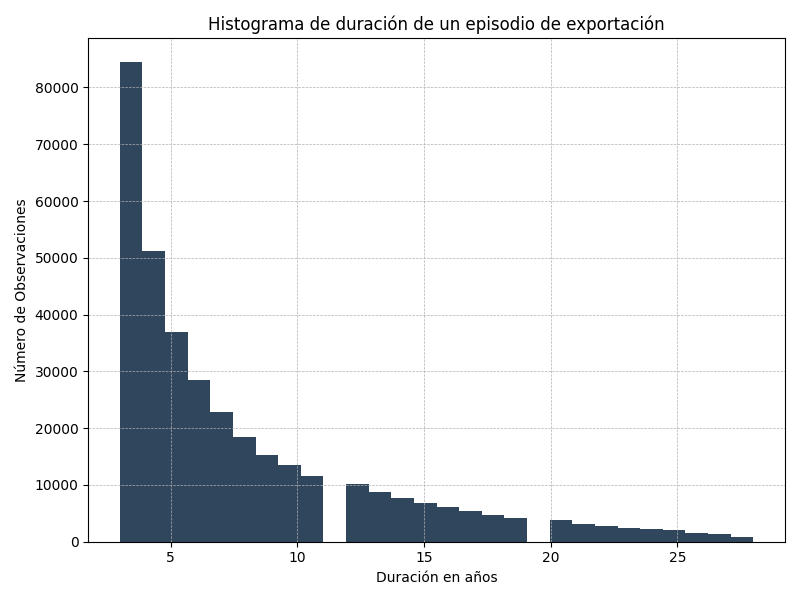
\includegraphics[width=0.6\textwidth]{Image1.png}
        \footnote{Se define un auge \textbf{sostenido} a partir de 3 años consecutivos de duración.}
    \end{center}
\end{frame}

\begin{frame}{Los episodios más duraderos están asociados con mayores incrementos en exportaciones}
    \begin{center}
        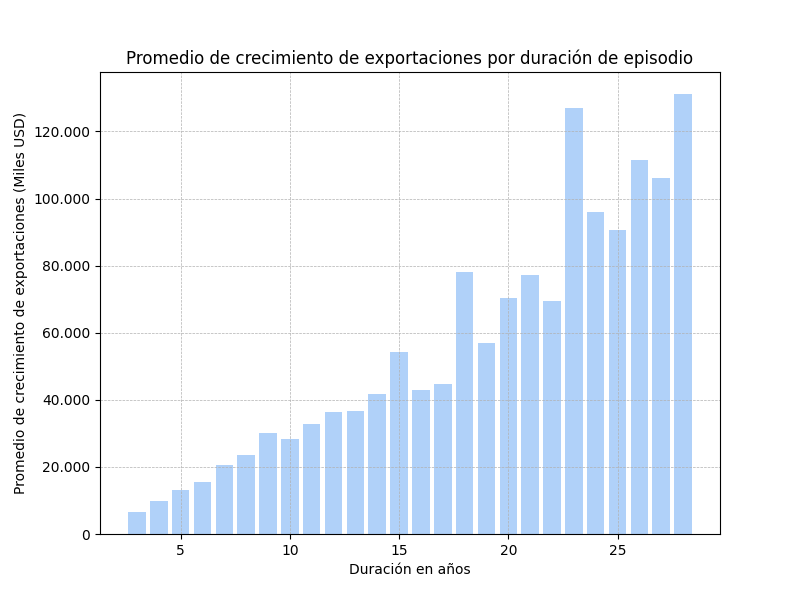
\includegraphics[width=0.6\textwidth]{Image2.png}
    \end{center}
\end{frame}

%==================================
% BLOQUE 2 — Estimación y proyección del modelo GLM
%==================================
\begin{frame}{Estructura general de la metodología}
    \begin{enumerate}
        \item \textcolor{gray!70}{Identificación de episodios de exportación}
        \item \textbf{Estimación y proyección del modelo GLM}
        \item \textcolor{gray!70}{Análisis de PIB con la MIO y Valor Agregado}
        \item \textcolor{gray!70}{Cálculo de la oportunidad en pobreza y empleo}
    \end{enumerate}
\end{frame}

\begin{frame}{Estimación del modelo de crecimiento exportador}
    \begin{itemize}
        \item Este bloque modela características identificadas y medibles de los episodios de auge exportador para identificar los factores estructurales asociados a expansiones sostenidas en las exportaciones bilaterales por producto.
        \item Se estima un modelo lineal generalizado (GLM) con distribución Poisson y enlace logarítmico, adecuado para capturar la naturaleza no negativa y asimétrica de las variaciones en exportaciones.
        \item El modelo se estima sobre una base internacional (excluyendo a Colombia) para identificar regularidades empíricas entre países y productos, lo que permite posteriormente proyectar los cambios esperados en las exportaciones colombianas bajo escenarios contrafactuales comparables.
    \end{itemize}
\end{frame}

\begin{frame}{Estructura del modelo econométrico}
    \begin{itemize}
        \item Se utiliza un \textbf{modelo lineal generalizado (GLM)} con familia \textit{Poisson} y enlace \textit{log}, adecuado para modelar tasas de crecimiento no negativas y distribuciones asimétricas. Los errores se corrigen mediante varianzas robustas (\textbf{HC3}) para controlar heterocedasticidad.
        \item La especificación relaciona el cambio en exportaciones con variaciones en la demanda externa, la participación inicial del exportador, la distancia geográfica, el tamaño económico de los países, la afinidad cultural y los efectos sectoriales.
        \item La combinación de estas variables permite capturar tanto las condiciones de mercado (demanda y tamaño) como los factores estructurales que influyen en la competitividad exportadora y la expansión geográfica de las firmas.
        \item Se obtienen los parámetros estimados que se utilizan en la etapa de proyección para Colombia.
    \end{itemize}
\end{frame}

\begin{frame}{Especificación del modelo econométrico}
Para $t_0$ y $t^* = t_{t+1}$ con $t_0, t_{t+1} \in T$:
\begin{equation}
\Delta x_{o,d,p,t_0 \rightarrow t^*} =
\beta_0 + \beta_1 \times \Delta m_{d,p,t_0 \rightarrow t^*} +
\beta_2 \times s_{o,d,p,t_0} +
\end{equation}
\begin{equation*}
\delta_1 \times \log \text{distancia}_{o,d} +
\delta_2 \times \text{cultura}_{o,d} +
\delta_3 \times \text{industria}_p +
\end{equation*}
\begin{equation*}
\delta_4 \times \log \text{gdp}_{o,t} +
\delta_5 \times \log \text{gdp}_{d,t} +
\delta_6 \times \log \text{gdp}_{o,t}^2 +
\delta_7 \times \log \text{gdp}_{d,t}^2 +
\end{equation*}
\begin{equation*}
\delta_8 \times \log (t^*-t_0+1) +
\delta_9 \times \log (t^*-t_0+1)^2 +
\end{equation*}
\begin{equation*}
\phi_1 \times \text{región}_o +
\phi_2 \times \text{región}_d +
\varepsilon_{o,d,p,t_0 \rightarrow t^*}
\end{equation*}
\end{frame}

\begin{frame}{Controles incluidos en la especificación}
    \begin{itemize}
        \item \textbf{Distancia geográfica (log\_distancia):} proxy de los costos de transporte y las fricciones logísticas entre países origen y destino. CEPII.
        \item \textbf{Afinidad cultural (cultura\_similaridad):} captura la similitud institucional, lingüística o histórica entre socios comerciales, que reduce barreras de entrada.
        \item \textbf{Grupos de industria del producto (industria $x$):} controla diferencias tecnológicas y de estructura productiva según la clasificación CIIU. DANE.
        \item \textbf{PIB de origen y destino (log\_gdp\_o y log\_gdp\_d):} representan el tamaño y la capacidad económica de los países, permitiendo identificar no linealidades en el efecto del ingreso. Dólares PPP reales de 2019. IMF.
        \item \textbf{Duración del episodio (log\_duracion):} controla la extensión temporal del auge exportador.
        \item \textbf{Regiones de origen y destino (región\_o y región\_d):} dummies regionales según el geoesquema de Naciones Unidas, que capturan efectos espaciales y heterogeneidad estructural.
    \end{itemize}
\end{frame}

\begin{frame}{Proyección exportaciones para Colombia en 2025-2035}
    \begin{itemize}
        \item La predicción fuera de muestra busca estimar el cambio esperado en exportaciones colombianas aplicando los parámetros del modelo estimado con datos internacionales a las condiciones estructurales de Colombia.
        \item Este ejercicio permite evaluar cómo se comportaría Colombia si enfrentara un episodio de expansión exportadora con características similares a las observadas en otros países.
        \item Para realizar la proyección, se replica la estructura del conjunto de entrenamiento: se generan las mismas variables explicativas utilizadas en la estimación asegurando consistencia en definiciones y escalas.
        \item La duración del episodio se fija en 10 años (la mediana de la distribución de duración de un episodio).
    \end{itemize}
\end{frame}

\begin{frame}{Tratamiento de datos para la proyección fuera de muestra del modelo para el caso colombiano}
Se replica la estructura exacta del conjunto de entrenamiento, con los datos para Colombia:
  \begin{itemize}
    \item Calcular la cuota de mercado de Colombia en 2023 para cada producto recibido e identificado.
    \item Para bienes que Colombia aún no exporta: la cuota inicial es cero.
    \item Proyectar la demanda de los principales importadores a 2035 usando alisamiento exponencial.
    \begin{itemize}
        \item La proyección dependerá de el periodo promedio que dure un episodio. 
        \item Se hace para 65 países y 809 productos. Se eliminan observaciones vacías.
    \end{itemize}
    \item Aplicar los coeficientes estimados en la ecuación \textbf{(1)} para obtener el aumento potencial de exportaciones por producto e industria.
  \end{itemize}
\end{frame}

\begin{frame}{Resultados de la estimación del modelo econométrico}
    \begin{center}
        \scriptsize
        \begin{tabular}{lr}
        \toprule
        Variable & Coeficiente \\
        \midrule
        const & -2.9310 \\
        log\_Delta\_m & 0.1141 \\
        share\_start & 1.8564 \\
        log\_duracion & 2.0751 \\
        log\_duracion2 & -0.2205 \\
        log\_gdp\_o & 0.0923 \\
        log\_gdp\_o2 & -0.0008 \\
        log\_gdp\_d & 0.6830 \\
        log\_gdp\_d2 & -0.0092 \\
        log\_distancia & -0.3117 \\
        cultura\_similaridad & -0.0103 \\
        industria\_26 - Otros & 1.9175 \\
        industria\_Otras industrias & 1.9856 \\
        \bottomrule
        \end{tabular}
    \end{center}
\end{frame}

\begin{frame}{Porcentaje de éxito exportador en la proyección}
    \begin{itemize}
        \item Al aplicar el modelo de proyección a todos los productos y destinos con demanda potencial, se asume implícitamente que Colombia podría exportar exitosamente a todos los mercados, sin restricciones productivas, logísticas ni institucionales.
        \item Este supuesto resulta poco realista: en la práctica, solo una fracción de los productos logra consolidar un episodio de crecimiento sostenido en las exportaciones.
        \item Para aproximar un escenario más plausible, se estima la {proporción de productos que efectivamente alcanzan un auge exportador} en países comparables a Colombia.
        \item Esta proporción se estima como referencia empírica del éxito exportador observado. El escenario base del modelo no la aplica como ponderador: el \textit{bootstrap} remuestrea una fracción fija de los productos proyectados, del 15\%, y de ahí salen los {intervalos de confianza y las exportaciones esperadas}.
    \end{itemize}
\end{frame}


\begin{frame}{Estimación de la proporción de productos exitosos en países comparables}
    \begin{itemize}
        \item Se mide, para México, Costa Rica y República Dominicana, la proporción de productos que cumplen la primera condición de \textit{Freund \& Pierola (2008)}: un episodio de crecimiento exportador hacia Estados Unidos con incremento medio anual superior al 6\%.
        \item Esta condición se adopta como una {medida simplificada de éxito exportador}, dado que captura la capacidad de un producto para sostener una expansión significativa durante varios años consecutivos.
        \item En la práctica, los países no son exitosos en todos sus productos ni mercados. Por eso, estimar esta proporción permite ajustar la proyección colombiana a una {tasa de éxito empírica observada}.
        \item La proporción se define como \(\pi_o = \frac{\sum_{p \in P_{d \rightarrow o}} \mathbf{1}\{p,o \text{ tiene episodio}\}}{|P_{d \rightarrow o}|}\), y los resultados obtenidos fueron: México 54.4\%, Costa Rica 20.4\% y República Dominicana 26.6\%, con un promedio de 33.8\%.
    \end{itemize}
\end{frame}

\begin{frame}{Posteriormente, realizamos un procedimiento de \textit{bootstrap} para capturar la incertidumbre en los resultados}
    \begin{itemize}
        \item La idea es aproximar, mediante simulación, los posibles resultados que surgirían si distintos subconjuntos de productos fueran exitosos, manteniendo la estructura general del modelo.
        \item El \textit{bootstrap} se utiliza para evaluar la incertidumbre asociada al hecho de que no todos los productos proyectados alcanzan efectivamente un episodio de auge exportador.  
        \item En cada una de las iteraciones, se realiza un remuestreo aleatorio con reemplazo del conjunto de proyecciones, seleccionando la proporción de productos correspondiente a cada escenario.
        \item Se definen tres escenarios conservadores de éxito: conservador (10\%), base (15\%) y optimista (20\%), que representan la fracción de productos que materializan un crecimiento sostenido.
    \end{itemize}
\end{frame}

\begin{frame}{Ventajas estadísticas y utilidad del procedimiento de \textit{bootstrap}}
    \begin{itemize}
        \item Cada submuestra constituye una versión alternativa del escenario exportador, lo que permite generar una distribución empírica de resultados para las exportaciones, el PIB y otras variables de interés.
        \item Permite obtener medidas de dispersión e incertidumbre sin asumir una forma funcional o distribución específica de los errores.
        \item Refleja la variabilidad real de los datos y proporciona estimaciones más robustas frente a valores atípicos o muestras pequeñas.
        \item Los intervalos de confianza derivados de las simulaciones representan el rango dentro del cual se espera que se ubiquen las verdaderas magnitudes de exportaciones y PIB bajo distintos escenarios de éxito.
    \end{itemize}
\end{frame}

%----------------------------------
% 1. Exportaciones proyectadas a 2045
%----------------------------------
\begin{frame}
\frametitle{¿Cómo crecen las exportaciones en un auge exportador exitoso?}

\vspace{0.3cm}
\begin{itemize}
    \item Se desarrolló un índice normalizado que captura la forma funcional del \textbf{crecimiento de exportaciones en 20 años}, utilizando información histórica de \textbf{Colombia, México, Costa Rica y República Dominicana}.
    \begin{itemize}
        \item Se calcula sobre 20 años para describir la dinámica del auge exportador siendo conservadores en su duración.
    \end{itemize}
    \item Cada serie histórica se transformó a índice base 1, donde el primer año de cada ventana temporal se establece como referencia (índice = 1.0). El promedio extrae \textbf{el patrón común de crecimiento observado}.
    
    \item El índice representa la forma \textbf{funcional típica}: no una tasa constante, sino una trayectoria con dinámicas observadas históricamente.
\end{itemize}

\end{frame}

\begin{frame}{Estructura de los Datos}

\begin{itemize}
    \item Los datos se obtuvieron de la base de datos de comercio internacional de la \textbf{UN Comtrade}.
    \item Para el análisis se utilizan las exportaciones totales desagregadas por país y año. 
    \item Las variables principales que componen esta base incluyen 
    \begin{itemize}
        \item \texttt{ReporterName} que identifica el nombre del país exportador
        \item \texttt{Year} que corresponde al año de la observación
        \item \texttt{TradeValue in 1000 USD} que registra el valor de las exportaciones expresado en miles de dólares estadounidenses.
    \end{itemize}
    \item El período de análisis abarca desde la década de 1990 hasta 2025, específicamente:
    \begin{itemize}
        \item   Colombia: 1990--2024
        \item   México: 1990--2024
        \item   Costa Rica: 1994--2023
        \item   República Dominicana: 1996--2023 (Vacío entre 1996 y 2001)
    \end{itemize} 
\end{itemize}

\end{frame}

\begin{frame}{Comportamiento de las Exportaciones}
\begin{figure}
    \centering
    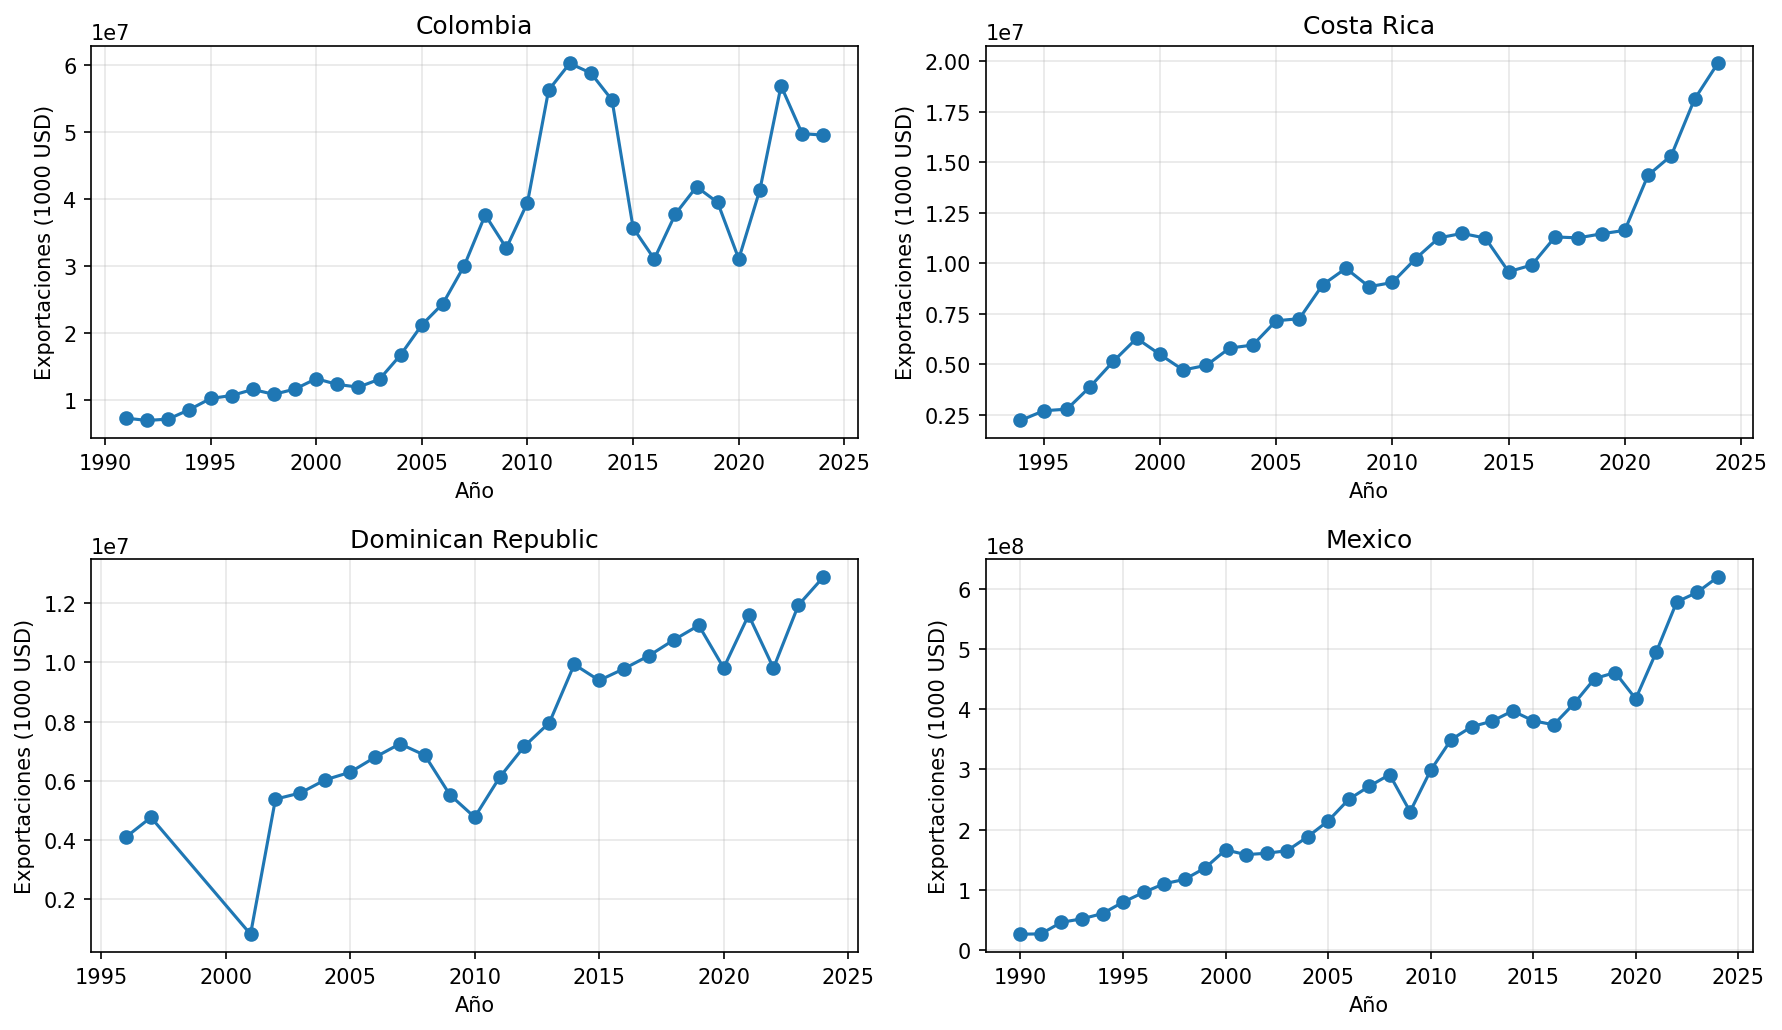
\includegraphics[width=0.7\textwidth]{expos.png}
    \caption{Series temporales de exportaciones para cada país}
\end{figure}
\end{frame}

\begin{frame}{Metodología: Paso 1 - Normalización}

Para cada país $i$ y cada año $t$, se observa el valor de exportaciones $X_{i,t}$.

\vspace{0.3cm}

\textbf{Normalización a índice base 1:}

Para cada ventana temporal que comienza en el año $t_0$ y termina en $t_0 + 19$:

\[I_{i,t} = \frac{X_{i,t}}{X_{i,t_0}}\]

donde $I_{i,t_0} = 1$ por construcción.

\vspace{0.3cm}

\textbf{Interpretación:} El índice $I_{i,t}$ representa el factor de crecimiento acumulado desde el año base. Por ejemplo, $I_{i,t} = 2.5$ indica que las exportaciones se han multiplicado por 2.5 respecto al año inicial.

\end{frame}

\begin{frame}{Metodología: Paso 2 - Ventanas Móviles}

\textbf{Ventanas móviles (rolling windows):}

Para cada país $i$ con $T_i$ años de datos, se construyen múltiples ventanas de 20 años:

\vspace{0.3cm}

\begin{itemize}
    \item Ventana 1: años $[t_1, t_1+19]$
    \item Ventana 2: años $[t_2, t_2+19]$
    \item $\vdots$
    \item Ventana $W_i$: años $[t_{W_i}, t_{W_i}+19]$
\end{itemize}

\vspace{0.3cm}

donde $W_i = T_i - 19$ es el número total de ventanas para el país $i$.

\vspace{0.3cm}

\textbf{Resultado:} Cada ventana genera una trayectoria normalizada de 20 puntos: $\{I_{i,w,0}, I_{i,w,1}, \ldots, I_{i,w,19}\}$ donde $w$ indexa la ventana.

\end{frame}

\begin{frame}{Metodología: Paso 3 - Promedio de Índices}

\textbf{Índice promedio entre países y ventanas:}

Para cada período $s \in \{0, 1, 2, \ldots, 19\}$:

\[\bar{I}_s = \frac{1}{N} \sum_{i=1}^{K} \sum_{w=1}^{W_i} I_{i,w,s}\]

donde:
\begin{itemize}
    \item $K$ = número de países
    \item $W_i$ = número de ventanas del país $i$
    \item $N = \sum_{i=1}^{K} W_i$ = número total de observaciones
\end{itemize}

\vspace{0.3cm}

\textbf{Resultado:} Vector de 20 valores $\{\bar{I}_0, \bar{I}_1, \ldots, \bar{I}_{19}\}$ que representa la trayectoria promedio de crecimiento para cada ventana.

\end{frame}

\begin{frame}{Justificación del Promedio de Índices}

El promedio cumple tres funciones estadísticas fundamentales:

\vspace{0.3cm}

\begin{enumerate}
    \item \textbf{Identificación del patrón común:} Identifica la forma funcional media del crecimiento de exportaciones, eliminando fluctuaciones específicas de cada país o período.
    
    \vspace{0.2cm}
    
    \item \textbf{Robustez:} Reduce el impacto de observaciones atípicas y eventos idiosincráticos (crisis, booms temporales).
    
    \vspace{0.2cm}
    
    \item \textbf{Generalización:} Permite aplicar el índice al contexto colombiano, asumiendo que la dinámica subyacente del crecimiento de exportaciones es similar entre economías comparables, sin dejar de tener en cuenta la dinámica observada del país.
\end{enumerate}

\end{frame}

\begin{frame}{Se aplican los Índices Normalizados sobre las proyecciones exportadoras}
\begin{itemize}
    \item El índice normalizado se aplica a  las proyecciones de exportaciones, tanto vegetativas como ganancia potencial, mediante reescalado, que preserva la forma funcional observada históricamente.
    \item Se definen un valor inicial $x_0$ (proyección de exportaciones en el año base) y un valor final $x_{19}$ (meta en 20 años). El crecimiento total objetivo es $(x_{19} - x_0)$.
    \item Para cada período $t$, el índice indica qué proporción del crecimiento total se había alcanzado históricamente.
    \item La fórmula de reescalado distribuye el crecimiento objetivo siguiendo la dinámica temporal capturada en el índice histórico:
    \begin{center}

        $\displaystyle \bar{X}_t = x_0 + (x_{19} - x_0) \times \left[\frac{(i_t - 1)}{(i_{19} - 1)}\right]$
    \end{center}
    \item Posteriormente, para mantener un prónostico conservador, pormediamos la senda modelada con una senda estimada de forma exponencial para suavizar la volatilidad de las trayectorias.
\end{itemize}
\end{frame}

\begin{frame}{Como resultado, desarrollar la estrategia conllevaría a 122.650 USD mill. en exportaciones adicionales en este año, en el escenario base}
    \begin{columns}[T]
        \begin{column}{0.58\textwidth}
            \begin{itemize}
                \item El valor adicional en exportaciones derivado del crecimiento exportador equivale a 15\% del PIB en 2045.
                \item Esto implicaría multiplicar las exportaciones no tradicionales entre 2025 y 2045 en aproximadamente 7 veces, y las exportaciones totales en 4 veces.
                \item En términos per cápita, el las exportaciones en Colombia pasarían de 900 USD en 2024 a 3.858 USD en 2045.
            \end{itemize}
        \end{column}
        \begin{column}{0.42\textwidth}
            \centering
            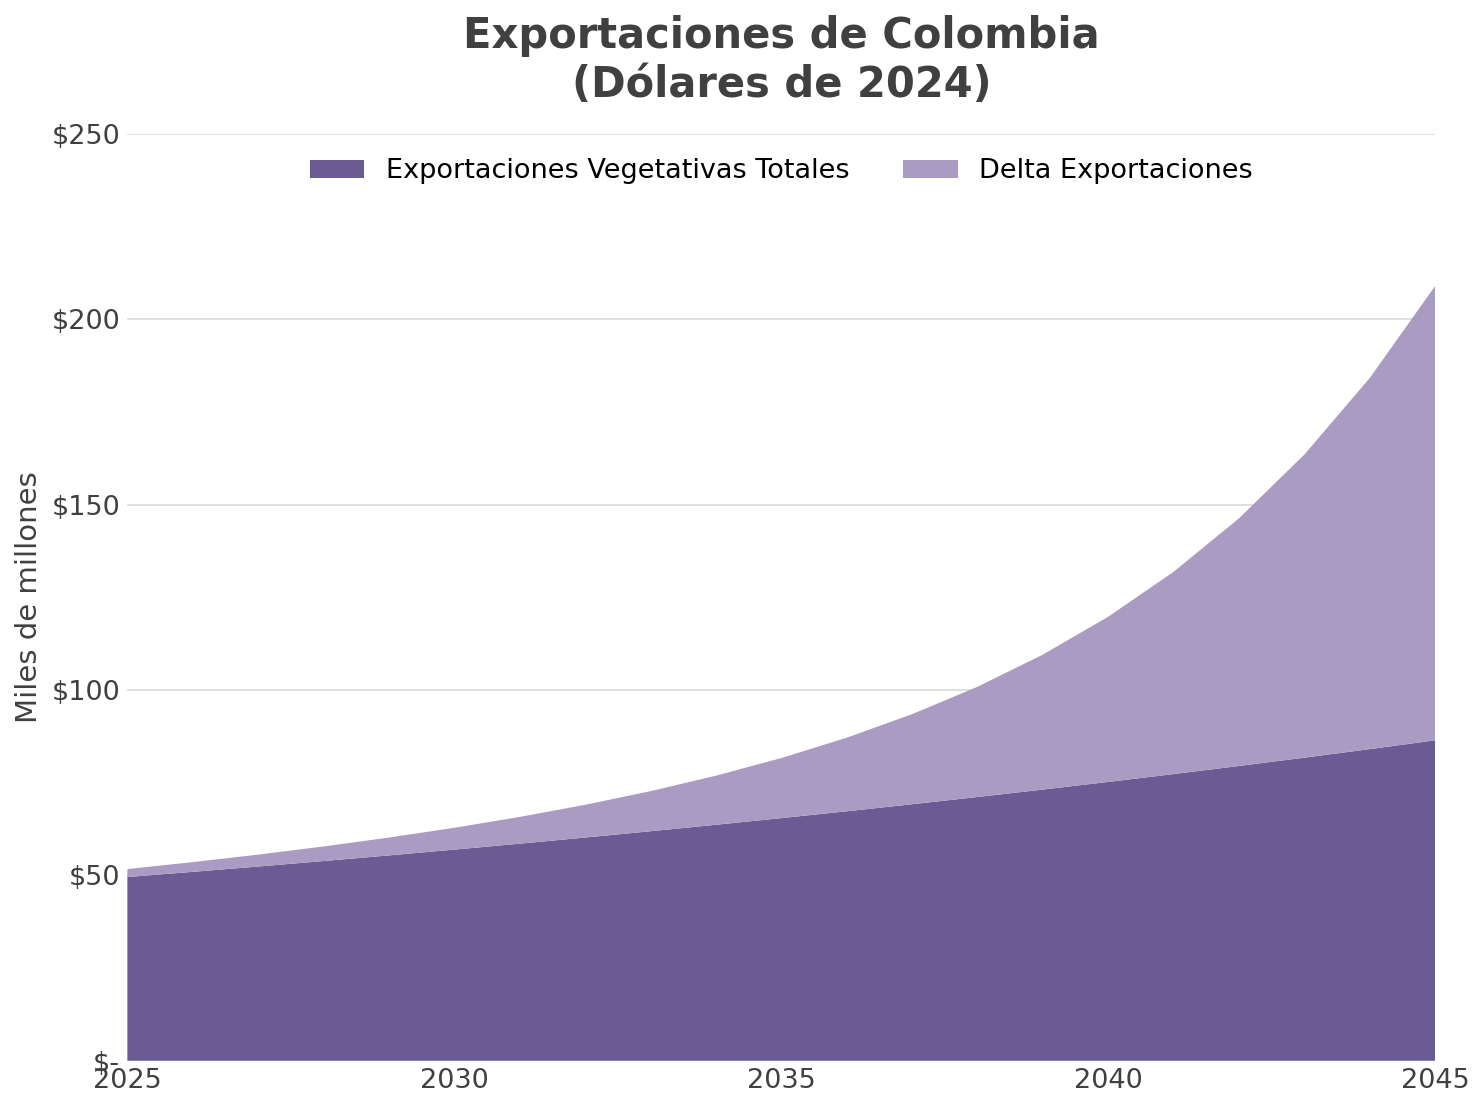
\includegraphics[width=\linewidth]{Imagen 1.png}
            \vspace{0.2cm}
            
            \tiny Fuente: Fedesarrollo
        \end{column}
    \end{columns}
\end{frame}

%==================================
% BLOQUE 3 — Análisis de PIB con la MIO y Valor Agregado
%==================================
\begin{frame}{Estructura general de la metodología}
    \begin{enumerate}
        \item \textcolor{gray!70}{Identificación de episodios de exportación}
        \item \textcolor{gray!70}{Estimación y proyección del modelo GLM}
        \item \textbf{Análisis de PIB con la MIO y Valor Agregado}
        \item \textcolor{gray!70}{Cálculo de la oportunidad en pobreza y empleo}
    \end{enumerate}
\end{frame}

\begin{frame}{Para medir esa oportunidad, utilizamos la metodología de Matriz Insumo–Producto}
    \begin{itemize}
        \item La Matriz Insumo–Producto (MIO) del DANE permite representar cómo los sectores de la economía colombiana están conectados entre sí, mostrando qué industrias compran y venden bienes y servicios a otras.
        \item En el contexto de este estudio, la MIO se utiliza para cuantificar cómo un choque positivo en la demanda externa se traduce en un aumento de producción, valor agregado y, finalmente, del PIB nacional.
        \item La metodología ofrece una visión integral de la oportunidad macroeconómica de un auge exportador, considerando los encadenamientos productivos y la estructura sectorial propia de la economía colombiana.
    \end{itemize}
\end{frame}

\begin{frame}{Estimamos el potencial efecto del auge exportador sobre la economía colombiana}
    \begin{itemize}
        \item Este bloque analiza cómo el crecimiento de las exportaciones se traduce en mayor producción y actividad económica dentro del país.
        \item Para hacerlo, se utiliza la Matriz de multiplicadores de Leontief obtenidas de la Matriz Insumo–Producto del DANE, que permite observar cómo los sectores están interconectados y cómo un aumento en la demanda externa se propaga por toda la economía.
        \item A partir de esta matriz, se estiman los efectos directos en las industrias exportadoras y los efectos indirectos sobre sus proveedores nacionales.
        \item Se incorporan los coeficientes de valor agregado para convertir el aumento en producción en una estimación de la oportunidad sobre el PIB, diferenciando su contribución por sector y capturando valores año a año.
    \end{itemize}
\end{frame}



\begin{frame}{Cómo representamos la distribución del producto en la economía colombiana}
  \textbf{1. Perspectiva por filas – Distribución del producto}
  \[
    \mathcal{X}_i = \sum_{j=1}^{n} x_{ij} + \mathcal{Y}_i
  \]
  \begin{itemize}
    \item $\mathcal{X}_i$: producción total generada por el sector $i$.
    \item $x_{ij}$: ventas del sector $i$ al sector $j$, reflejan la demanda intermedia dentro de la economía.
    \item $\mathcal{Y}_i$: demanda final del sector $i$ (consumo, inversión, gasto público, exportaciones netas).
    \item En nuestro caso, el aumento de exportaciones se incorpora dentro de $\mathcal{Y}_i$, representando el choque externo que impulsa la economía. Además, consideramos sector como industria CIIU.
  \end{itemize}
\end{frame}

\begin{frame}{Cómo interpretamos los requerimientos productivos de cada sector}
  \textbf{2. Perspectiva por columnas – Requerimientos de producción}
  \[
    \mathcal{X}_j = \sum_{i=1}^{n} x_{ij} + \mathcal{V}_j
  \]
  \begin{itemize}
    \item $\mathcal{X}_j$: producción total necesaria para abastecer la demanda del sector $j$.
    \item $x_{ij}$: insumos que el sector $j$ compra al sector $i$, mostrando su dependencia productiva.
    \item $\mathcal{V}_j$: valor agregado (salarios, utilidades, impuestos netos) generado en $j$.
    \item En este estudio, esta perspectiva permite ver cómo un mayor nivel de exportaciones en ciertos sectores genera una reacción en cadena sobre los demás sectores que les proveen insumos.
  \end{itemize}
\end{frame}

\begin{frame}{Cómo se construye la matriz que describe la tecnología de producción nacional}
  \textbf{3.1 Definición de coeficientes técnicos}
  \[
    a_{ij} = \frac{x_{ij}}{\mathcal{X}_j}
  \]
  \begin{itemize}
    \item Cada $a_{ij}$ muestra cuántos pesos del insumo del sector $i$ se requieren para producir un peso en el sector $j$.
    \item Esta relación resume la estructura tecnológica de la economía y la intensidad con que los sectores dependen unos de otros.
    \item Esta matriz se obtiene directamente del DANE, que calcula las interacciones productivas en Colombia.
  \end{itemize}
\end{frame}

\begin{frame}{Cómo se construye la matriz que describe la tecnología de producción nacional}
  \textbf{3.2 Construcción de la matriz $\mathcal{A}$}
  \[
    \mathcal{A} = [a_{ij}]_{i,j=1,\dots,n}
  \]
  \begin{itemize}
    \item La matriz $\mathcal{A}$ se utiliza para capturar los efectos directos del cambio exportador sobre la producción nacional.
    \item En este trabajo, refleja cómo un aumento en exportaciones de sectores específicos se transmite al resto de la economía según su patrón de insumo–producto.
  \end{itemize}
\end{frame}

\begin{frame}{Cómo estimamos el efecto total del choque exportador sobre la producción}
  \textbf{4. Modelo de Leontief}
  \[
    \mathcal{X} = \mathcal{A}\mathcal{X} + \mathcal{Y}
  \]
  \[
    (I - \mathcal{A})\mathcal{X} = \mathcal{Y} \quad \Rightarrow \quad \mathcal{X} = (I - \mathcal{A})^{-1}\mathcal{Y}
  \]
  \begin{itemize}
    \item La matriz inversa $(I - \mathcal{A})^{-1}$ permite estimar el efecto total que un cambio en la demanda final, como el aumento exportador, tiene sobre la producción de todos los sectores.
    \item En nuestro caso, la demanda externa se introduce como el choque $\mathcal{Y}$ y se propaga por toda la economía a través de los encadenamientos productivos.
    \item Así se obtiene el incremento total de producción asociado al auge exportador y la distribución de sus beneficios entre industrias.
  \end{itemize}
\end{frame}

\begin{frame}{Medición del choque de exportaciones en el contexto insumo–producto}
    \textbf{1. Vector de choque exportador}
    \[
        \Delta \mathcal{Y} = [\Delta \mathcal{E}_1, \Delta \mathcal{E}_2, \dots, \Delta \mathcal{E}_n]'
    \]
    \begin{itemize}
        \item Cada componente $\Delta \mathcal{E}_i$ representa el incremento esperado de exportaciones del sector $i$, obtenido a partir del modelo econométrico.
        \item Este vector constituye el punto de partida del análisis, pues refleja la magnitud y composición del impulso externo que ingresa a la economía.
    \end{itemize}
\end{frame}

\begin{frame}{Medición del choque de exportaciones en el contexto insumo–producto}
    \textbf{2. Transmisión del choque a la producción total}
    \[
        \Delta \mathcal{X} = (I - \mathcal{A})^{-1} \Delta \mathcal{Y}
    \]
    \begin{itemize}
        \item $\Delta \mathcal{X}$ indica el cambio total en la producción de cada sector tras incorporar el nuevo nivel de exportaciones.
        \item $(I - \mathcal{A})^{-1}$ es la inversa de Leontief, que mide cómo un aumento en la demanda final se propaga a lo largo de los encadenamientos productivos.
        \item Este proceso permite descomponer los efectos del auge exportador en dos componentes: directos (sectores que exportan) e indirectos (sectores que les proveen insumos).
    \end{itemize}
\end{frame}

\begin{frame}{Conversión del aumento de producción en oportunidad sobre el PIB colombiano}
    \textbf{1. Cálculo de los coeficientes de valor agregado}
    \[
        VA = [v_1, v_2, \dots, v_n]' , \quad 
        v_j = \frac{\mathcal{V}_j}{\mathcal{X}_j}
    \]
    \begin{itemize}
        \item Cada coeficiente $v_j$ representa la proporción del valor agregado que el sector $j$ aporta por unidad de producción.
        \item El vector $v$ resume la estructura de generación de ingresos, salarios e impuestos dentro de la economía.
        \item En este contexto, se usa para identificar qué parte del incremento en producción se traduce efectivamente en un aumento del PIB.
    \end{itemize}
\end{frame}

\begin{frame}{Conversión del aumento de producción en oportunidad sobre el PIB colombiano}
    \textbf{2. Estimación de la oportunidad sobre el PIB}
    \[
        \Delta PIB = VA' \, \Delta \mathcal{X} = VA' (I - \mathcal{A})^{-1} \, \Delta \mathcal{Y}
    \]
    \begin{itemize}
        \item $\Delta \mathcal{X}$: cambio total en la producción obtenido del modelo de Leontief.  
        \item $\Delta \mathcal{Y}$: vector del aumento en exportaciones por sector.  
        \item $(I - \mathcal{A})^{-1}$: matriz inversa que refleja los encadenamientos productivos.  
        \item La expresión muestra cómo un choque exportador inicial se convierte en incremento del PIB, combinando interdependencias sectoriales y generación de valor agregado.
    \end{itemize}
\end{frame}

\begin{frame}{Integración con la MIO I/II}
    \begin{itemize}
        \item Para todas las submuestras del bootstrap, se utiliza los multiplicadores de Leontief basados en la Matriz Insumo–Producto (MIO) del DANE, con base 2015 y desagregación de 68 industrias.
        \item Se establece un mapeo entre códigos HS6 de comercio internacional, las clasificaciones CIIU Rev.4 y las ramas MIO equivalentes. Este emparejamiento permite vincular cada producto exportado con la industria nacional correspondiente.
        \item El incremento proyectado en exportaciones se agrega por rama MIO para obtener un vector de choques sectoriales, que representa el aumento potencial por cada producto exportado de la demanda externa por industria.
        \item Los montos se convierten de USD reales 2015 a pesos colombianos (COP 2015) usando la tasa promedio de cambio y deflactores de precios consistentes con las cuentas nacionales.
    \end{itemize}
\end{frame}

\begin{frame}{Integración con la MIO II/II}
    \begin{itemize}
        \item Este vector de choques en pesos constantes constituye la entrada principal para el cálculo del \(\Delta PIB\) mediante los multiplicadores de Leontief.
        \item En términos estadísticos, cada escenario del \textit{bootstrap} genera un vector de choques $\Delta \mathcal{Y}$, correspondiente al aumento proyectado de exportaciones por sector.
    \end{itemize}
\end{frame}

\begin{frame}{Cómo integramos el auge exportador al modelo insumo–producto}
    \begin{itemize}
        \item Se establece un mapeo entre códigos HS6 de comercio internacional, la clasificación CIIU Rev.4 y las ramas MIO, para vincular cada producto exportado con su industria nacional correspondiente.
        \item El incremento proyectado en exportaciones se agrega por rama MIO y se convierte de dólares a pesos colombianos constantes (COP 2015) mediante tasas de cambio y deflactores coherentes con las cuentas nacionales.
        \item Este vector sectorial $\Delta \mathcal{Y}$ constituye la entrada del modelo de Leontief y permite estimar cómo el auge exportador se traduce en mayor producción y valor agregado dentro de la economía colombiana.
    \end{itemize}
\end{frame}

\begin{frame}{Oportunidad sectorial y agregación macroeconómica del choque en exportaciones}
    \begin{itemize}
        \item El vector de choques en exportaciones por rama MIO se multiplica por la matriz de multiplicadores de Leontief \((I - A)^{-1}\), obteniendo el efecto total sobre la producción de cada industria. Este resultado incorpora tanto los efectos directos como los encadenamientos indirectos entre sectores.
        \item A partir del vector de producción total resultante, se aplican los coeficientes de Valor Agregado (VA) del DANE, que expresan la proporción de producción que se traduce en valor agregado bruto por industria.
        \item La suma de los \(\Delta VA_i\) sectoriales proporciona el \(\Delta PIB\) total asociado al choque exportador. Este valor se expresa en pesos constantes de 2015 para mantener coherencia con el resto del análisis macroeconómico.
    \end{itemize}
\end{frame}

\begin{frame}{Consolidamos los resultados del bootstrap para obtener intervalos de confianza de la oportunidad económica}
    \begin{itemize}
        \item Para identificar la incertidumbre, realizamos un conjunto de simulaciones independientes basadas en los diferentes escenarios del bootstrap, donde cada uno refleja una posible combinación de productos exitosos.
        \item Con las 1.000 submuestras de datos, se construyen distribuciones empíricas de las principales variables de interés: cambio en el PIB y en exportaciones.
        \item A partir de esas distribuciones se obtienen las medias y los intervalos de confianza al 95 por ciento (percentiles 2.5 y 97.5), que reflejan el rango estadísticamente probable de la oportunidad económica del auge exportador.
    \end{itemize}
\end{frame}

\begin{frame}{Al 2045, desarrollar la estrategia conllevaría a 113.800 USD mill. de PIB adicional en este año tomando en cuenta el efecto sobre toda la economía colombiana}
    \begin{columns}[T]
        \begin{column}{0.58\textwidth}
            \begin{itemize}
                \item El valor adicional en producción equivale a 16\% del PIB de 2045.
                \item El Valor Presente Neto (VPN) del valor agregado adicional entre 2025 y 2045 sería de 1.779 billones de USD.
                \item Ese valor agregado adicional equivale al 170\% del PIB de 2024.
            \end{itemize}
        \end{column}
        \begin{column}{0.42\textwidth}
            \centering
            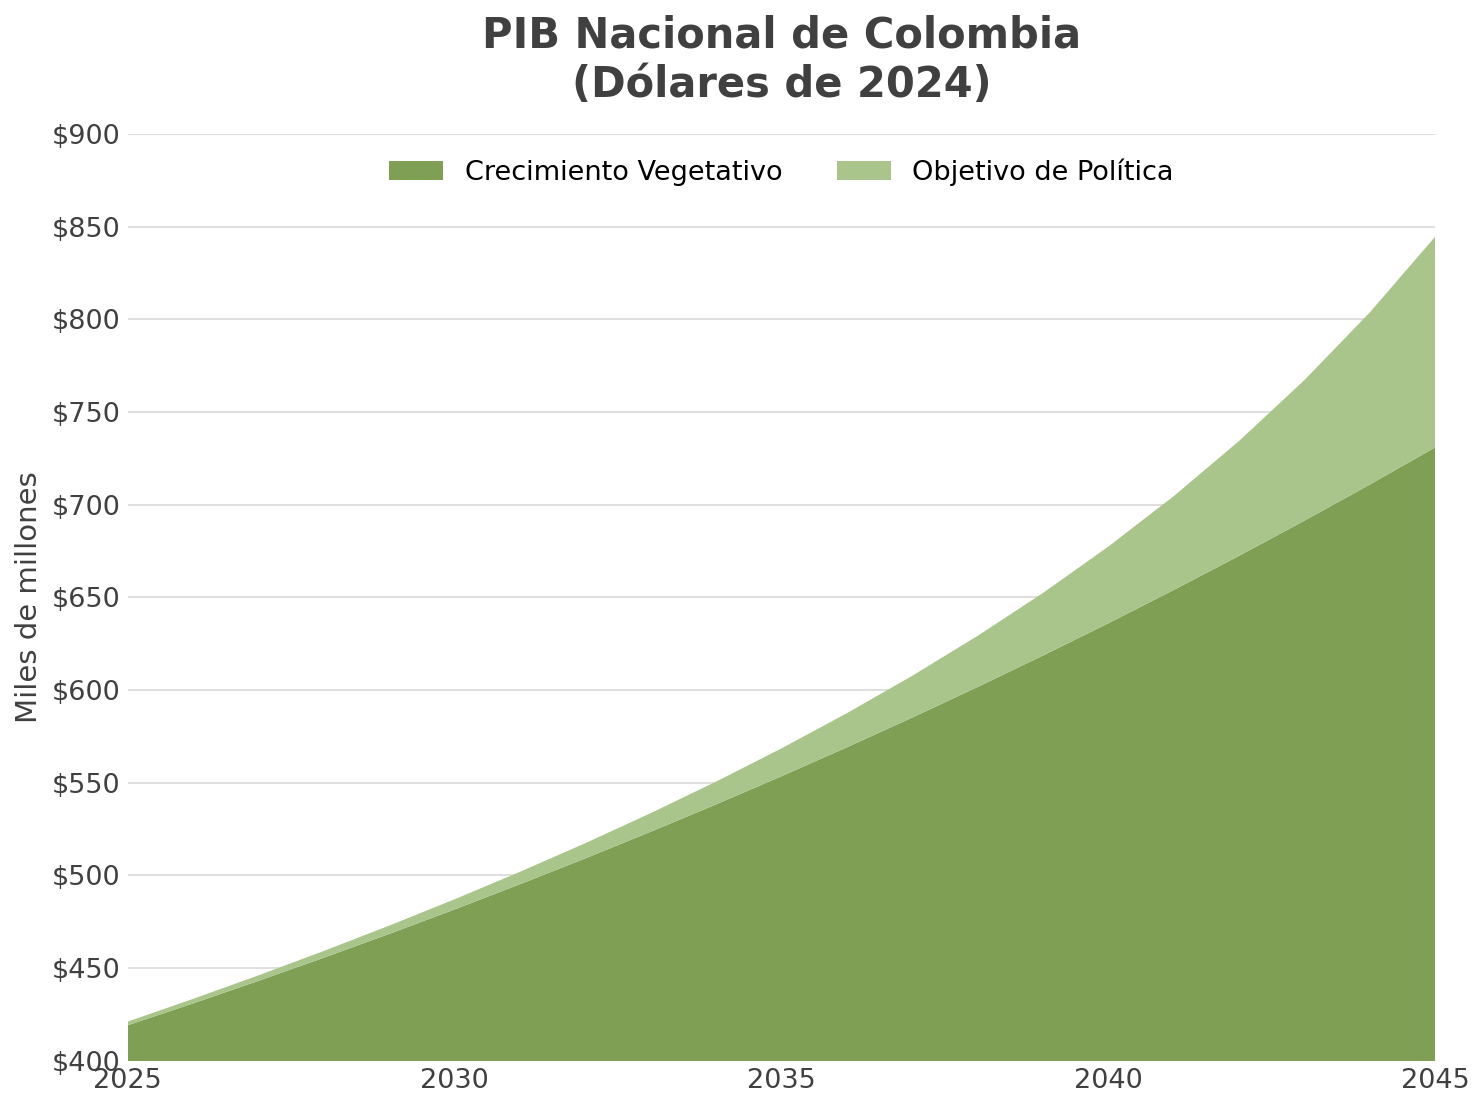
\includegraphics[width=\linewidth]{Imagen 2.png}
            \vspace{0.2cm}
            
            \tiny Fuente: Fedesarrollo
        \end{column}
    \end{columns}
\end{frame}

%----------------------------------
% 3. Proporción exportaciones/PIB
%----------------------------------
%\begin{frame}{Las posibles trayectorias de exportaciones como proporción del PIB}
%    \scriptsize
%    \begin{itemize}
%        \item En el escenario base, las exportaciones pasarían de representar 12\% del PIB en 2025 a 25\% en 2045. El rango de resultados oscila entre 21\% (escenario conservador) y 28\% (escenario optimista).
%    \end{itemize}
%    \vspace{0.3cm}
%    \centering
%    \includegraphics[width=0.6\linewidth]{Imagen 3.png}
%    \vspace{0.2cm}
%    
%    \tiny Fuente: Fedesarrollo
%\end{frame}

%==================================
% BLOQUE 4 — Cálculo de la oportunidad en pobreza y empleo
%==================================
\begin{frame}{Estructura general de la metodología}
    \begin{enumerate}
        \item \textcolor{gray!70}{Identificación de episodios de exportación}
        \item \textcolor{gray!70}{Estimación y proyección del modelo GLM}
        \item \textcolor{gray!70}{Análisis de PIB con la MIO y Valor Agregado}
        \item \textbf{Cálculo de la oportunidad en pobreza y empleo}
    \end{enumerate}
\end{frame}

\begin{frame}{Cómo traducimos la oportunidad económica en efectos sociales y fiscales}
    \begin{itemize}
        \item Este bloque traduce el incremento estimado del PIB, derivado del auge exportador, en oportunidads sociales y fiscales medibles sobre empleo, pobreza y recaudo.
        \item Se utilizan elasticidades macroeconómicas oficiales estimadas por el DANE, el equipo DAMS y el Ministerio de Hacienda, que permiten vincular los cambios en el PIB con variaciones en los indicadores sociales.
        \item Las estimaciones se aplican sobre los resultados del \(\Delta PIB\) obtenido en el análisis con la Matriz Insumo–Producto, garantizando consistencia entre la oportunidad económica y los efectos distributivos.
    \end{itemize}
\end{frame}

\begin{frame}{Elasticidades empleo–PIB y pobreza–PIB}
    \begin{itemize}
        \item \textbf{Elasticidad empleo/pobreza–PIB:} estimada por el equipo DAMS con base en datos de la Gran Encuesta Integrada de Hogares (GEIH) del DANE. Representa el cambio porcentual en empleo total ante un cambio de 1\% en el PIB real en el periodo anterior.
        \item Ambas elasticidades se aplican sobre el \(\Delta PIB\) sectorial y total derivado de la MIO, ponderando los resultados según la estructura de empleo y pobreza de 2024.
        \item Las estimaciones se expresan en términos absolutos (personas) y relativos (variación porcentual), para facilitar su interpretación en el contexto de política pública.
    \end{itemize}
\end{frame}

\begin{frame}{Traducción del crecimiento económico en empleo, reducción de pobreza y cambio en recaudo}
    \begin{itemize}
        \item A partir del \(\Delta PIB\) proyectado y las elasticidades oficiales, se estima la variación porcentual esperada en empleo total y en pobreza monetaria, diferenciando efectos en pobreza extrema y moderada.
        \item Los resultados se presentan como rangos con intervalos de confianza derivados del \textit{bootstrap} macroeconómico, reflejando la incertidumbre en las proyecciones del \(\Delta PIB\).
        \item Para el componente fiscal, se aplica la elasticidad ingreso–recaudo del Marco Físcal de Mediano Plazo 2024, Ministerio de Hacienda (2024), lo que permite estimar el aumento del recaudo tributario total asociado al crecimiento exportador.
    \end{itemize}
\end{frame}



%----------------------------------
% 4. Impacto social y fiscal
%----------------------------------
\begin{frame}{Del crecimiento económico a los resultados sociales y fiscales a 2045}

    \begin{columns}[T]
        \begin{column}{0.32\textwidth}
            \centering
            
            \textbf{Reducción del desempleo}
            \begin{itemize}
                \item Se lograría reincorporar a la población ocupada a 2,4 millones de personas.
                \item Esto equivale al 10,32\% de la población ocupada en diciembre de 2024.
            \end{itemize}
        \end{column}
        \begin{column}{0.32\textwidth}
            
            \textbf{Reducción de la pobreza}
            \begin{itemize}
                \item 3,4 millones de personas saldrían de la pobreza monetaria y 1,7 millones de la pobreza extrema.
                \item Representa reducciones de 21\% y 11\% sobre la población en pobreza monetaria y extrema, respectivamente.
            \end{itemize}
        \end{column}
        \begin{column}{0.32\textwidth}
            
            \textbf{Aumento del recaudo tributario}
            \begin{itemize}
                \item El crecimiento exportador aumentaría el recaudo total en 1.030 billones COP en VPN.
                \item Este valor equivale a 9,92\% del PIB de 2024.
            \end{itemize}
        \end{column}
    \end{columns}
\end{frame}

\begin{frame}
\frametitle{En los próximos 20 años, se estimó la oportunidad de política por periodo}

% Definir los colores necesarios
\definecolor{azulclaro}{RGB}{173, 216, 230}
\definecolor{grisclaro}{RGB}{220, 220, 220}

\vspace{0.2cm}
\begin{center}
\tiny
\renewcommand{\arraystretch}{1.2}
\begin{tabular}{|l|c|c|c|c|}
\hline
 & \textbf{Reducción del} & \multicolumn{2}{c|}{\textbf{Reducción de la Pobreza}} & \textbf{Aumento del} \\
 & \textbf{Desempleo} & \multicolumn{2}{c|}{} & \textbf{Recaudo Tributario} \\
\hline
\textbf{P1: 2025--2029} & \textbf{549,710 } \newline {\tiny (2.39\%)*} & \textbf{1.1M } \newline {\tiny (monetaria) (6.84\%)**} & \textbf{555 mil } \newline {\tiny (extrema) (3.42\%)**} & \textbf{\$18.7B} \newline {\tiny (1.80\%) PIB 2024} \\
\hline
\textbf{P2: 2030--2033} & \textbf{823,419 } \newline {\tiny (3.57\%)*} & \textbf{1.3M } \newline {\tiny (monetaria) (7.84\%)**} & \textbf{636 mil } \newline {\tiny (extrema) (3.92\%)**} & \textbf{\$23.2B} \newline {\tiny (2.29\%) PIB 2024} \\
\hline
\textbf{P3: 2034--2037} & \textbf{708,188 } \newline {\tiny (3.07\%)*} & \textbf{895 mil } \newline {\tiny (monetaria) (5.51\%)**} & \textbf{447 mil} \newline {\tiny (extrema) (2.75\%)**} & \textbf{\$24.2B} \newline {\tiny (2.33\%) PIB 2024} \\
\hline
\textbf{P4: 2038--2041} & \textbf{295,304 } \newline {\tiny (1.28\%)*} & \textbf{123 mil } \newline {\tiny (monetaria) (0.75\%)**} & \textbf{61 mil } \newline {\tiny (extrema) (0.38\%)**} & \textbf{\$21.5B} \newline {\tiny (2.07\%) PIB 2024} \\
\hline
\textbf{P5: 2042--2045} & \textbf{0}  & \textbf{0}  & \textbf{0}  & \textbf{\$14.5B} \newline {\tiny (1.4\%) PIB 2024} \\
\hline
\end{tabular}
\end{center}

\vspace{0.2cm}
{\scriptsize * \% de población ocupada en diciembre de 2024 \hspace{1cm} ** \% sobre la población en pobreza monetaria respectivamente}

\vspace{0.3cm}
{\footnotesize Fuente: Fedesarrollo}

\end{frame}

%\begin{frame}
%\frametitle
\begin{frame}
\frametitle{Adicionalmente, las industrias se priorizan según la proyección de demanda para los últimos años.}

Para estimar el potencial de demanda de cada CIIU de forma conservadora, se realiza una simulación que asume que solo una fracción de los productos logrará captar demanda.

\textbf{Notación:}
\begin{itemize}
    \item $\mathcal{P}_c$ = productos del CIIU $c$, cada uno con demanda $d_p$
    \item $D_c = \sum_{p \in \mathcal{P}_c} d_p$ = potencial total del CIIU
\end{itemize}

\textbf{Proceso (1,000 iteraciones):}

En cada iteración $k$:
\begin{enumerate}
    \item Seleccionar aleatoriamente 10-20\% de los productos de cada CIIU
    \item Sumar su demanda: \quad $D_c^{(k)} = \displaystyle\sum_{p \in \text{muestra}} d_p$
\end{enumerate}

\textbf{Resultado:} Promedio de las simulaciones $\bar{D}_c = \frac{1}{1000}\sum_{k} D_c^{(k)}$

\end{frame}

%===============================================
% LÁMINA 2: Construcción del Ranking
%===============================================
\begin{frame}
\frametitle{Construcción del Ranking}

\begin{itemize}
    \item \textbf{Ranking primario:} Los CIIUs se ordenan de mayor a menor según su potencial de demanda promedio $\bar{D}_c$.
    
    \item \textbf{Criterio de desempate:} En caso de empate, se prioriza el CIIU con más productos en el Top-5 de complejidad, proximidad, crecimiento o sostenibilidad.
    
    \item \textbf{Ranking final:} Se ordenan los CIIUs por $(\bar{D}_c, \text{productos Top-5})$ en orden descendente.
\end{itemize}

\textbf{¿Por qué simulación?}
\begin{itemize}
    \item \textbf{Conservador:} Asume éxito parcial (solo 10--20\% de productos captan demanda)
    \item \textbf{Robusto:} Reduce la influencia de productos con valores atípicos
    \item \textbf{Estable:} 1,000 réplicas garantizan resultados consistentes
\end{itemize}

\end{frame}

%===============================================
% LÁMINA 3: Resumen del Proceso
%===============================================
\begin{frame}
\frametitle{Se puede descomponer la proyección de ganancia exportadora por industrias}
\scriptsize
\begin{columns}[T]
\begin{column}{0.45\textwidth}
\begin{itemize}
    \item Se desagrega la ganancia exportadora entre las 10 industrias específicas identificadas, excluyendo la categoría agregada "Otros" que representa el restante 53\%.
    \item Pesca marítima lidera con el 24\% de las exportaciones específicas, seguida por Fabricación de vehículos automotores (13\%) e Industrias básicas de hierro y acero (11\%).
    \item Las proporciones entre industrias se mantienen constantes en cada período, lo que permite identificar claramente la contribución relativa de cada sector durante todo el horizonte de proyección.
\end{itemize}
\end{column}
\begin{column}{0.55\textwidth}
    \centering
    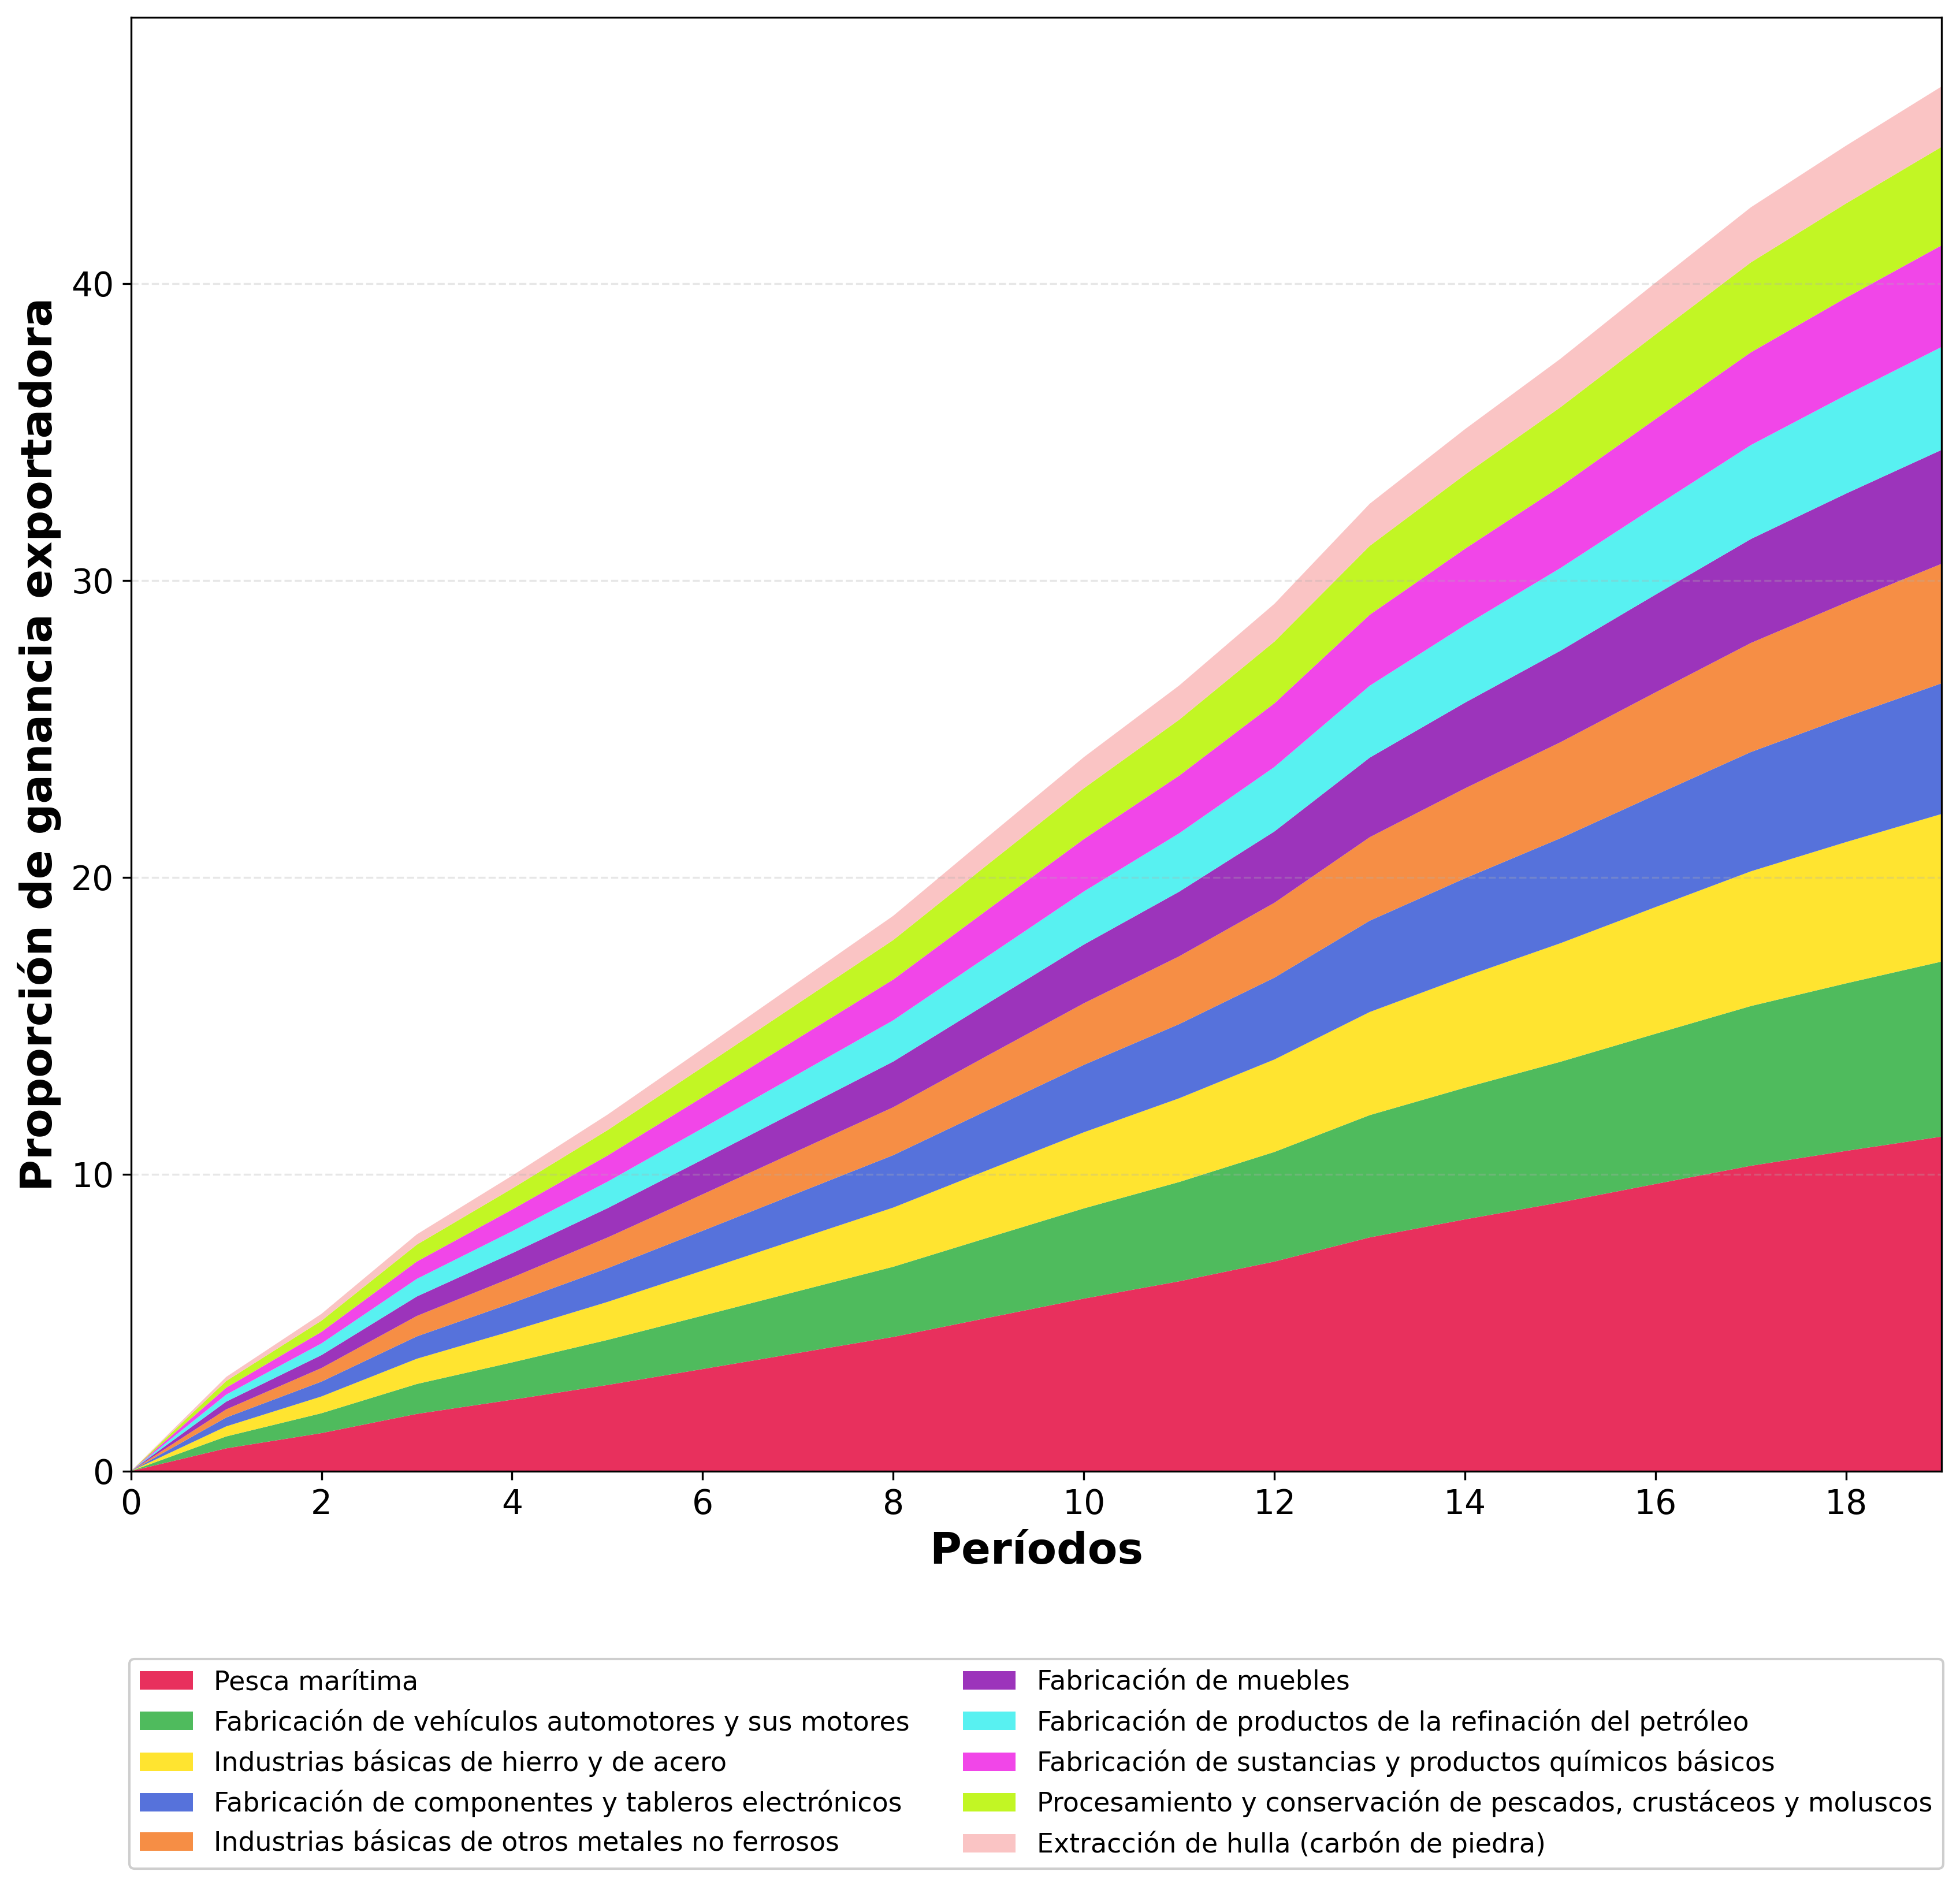
\includegraphics[width=\linewidth]{Imagen 4.png}
    \vspace{0.2cm}
    
    \tiny Fuente: Fedesarrollo
\end{column}
\end{columns}
\end{frame}


\begin{frame}
\frametitle{Priorización de Industrias según potencial exportadora}
\tiny
\renewcommand{\arraystretch}{1.2}
\begin{center}
\begin{columns}[T]
\begin{column}{0.48\textwidth}
\centering
\begin{tabular}{lrr}
\toprule
Industria & Part. & Prod. \\
\midrule
Industria de maquinaria y transporte & 22.63\% & 123 \\
Productos equipos de potencia y distribución eléctrica & 16.01\% & 67 \\
Metales derivados de materiales reciclados & 12.25\% & 79 \\
Sector farmacéutico & 6.27\% & 99 \\
Otros & 6.25\% & 17 \\
Textiles y confección & 5.16\% & 60 \\
Derivados petróleo básicos & 4.34\% & 10 \\
Minería & 4.30\% & 23 \\
Madera & 3.60\% & 3 \\
Plásticos y caucho & 2.61\% & 35 \\
Papel y productos de papel & 2.46\% & 11 \\
Otros productos alimenticios & 2.40\% & 22 \\
\bottomrule
\end{tabular}
\end{column}
\begin{column}{0.48\textwidth}
\centering
\begin{tabular}{lrr}
\toprule
Industria & Part. & Prod. \\
\midrule
Frutas frescas y frutas procesadas & 2.28\% & 25 \\
Química básica & 1.70\% & 27 \\
Metales a partir de material recuperado & 1.22\% & 4 \\
Minerales no metálicos & 1.05\% & 7 \\
Azúcar y derivados primarios & 0.87\% & 1 \\
Cosméticos y productos de aseo personal & 0.86\% & 11 \\
Cafés y cafes especiales & 0.85\% & 3 \\
Pesca y acuicultura & 0.65\% & 3 \\
Confitería & 0.62\% & 6 \\
Carne bovina & 0.61\% & 13 \\
Agroquímicos y biológicos & 0.53\% & 3 \\
Productos metálicos & 0.51\% & 10 \\
\bottomrule
\end{tabular}
\end{column}
\end{columns}
\end{center}
\end{frame}

\end{document}